% This must be in the first 5 lines to tell arXiv to use pdfLaTeX.
\pdfoutput=1

\documentclass[11pt]{article}

% "final" drops review line numbers and shows the named author. "nohyperref" keeps
% this ACL2023 template compatible with the local Tectonic/XeTeX build.
\usepackage[final,nohyperref]{ACL2023}

% ACL2023.sty insets the abstract by 0.6cm on each side on top of the page
% margins; override with a smaller inset so it reads at nearly full column width.
\makeatletter
\renewenvironment{abstract}%
    {\vspace{-0.15cm}\centerline{\large\bf Abstract}%
     \begin{list}{}%
        {\setlength{\rightmargin}{0.1cm}%
         \setlength{\leftmargin}{0.1cm}}%
      \item[]\ignorespaces%
      \@setsize\normalsize{12pt}\xpt\@xpt
      }%
    {\unskip\end{list}}
\makeatother

\usepackage{times}
\usepackage{latexsym}
\usepackage{amsmath,amssymb}
\usepackage[capitalize]{cleveref}

\usepackage[T1]{fontenc}
\usepackage[utf8]{inputenc}

\usepackage{microtype}
\usepackage{inconsolata}

% Uniform inter-word spacing: without this, LaTeX adds extra stretchable space
% after any period it guesses ends a sentence, which reads as distractingly wide
% gaps once text is justified in a narrow two-column layout.
\frenchspacing

\usepackage{graphicx}
\usepackage{booktabs}
\usepackage{float}
\usepackage{xcolor}

\graphicspath{{figures/}}

% Deliberately loud: any empirical claim still awaiting the final grid numbers is
% marked so it cannot be missed in a page-through before submission. Grep for
% "TODO" in this file, or search the PDF, to find every remaining slot.
\newcommand{\TODO}[1]{\textcolor{red}{\textbf{[TODO: #1]}}}

\title{Generative Latent Models for DeepSDF:\\
Gaussian vs.\ Diffusion in the Small-Data Regime}
\author{Amit Benbenishti \\
  Deep Learning for 3D Computer Vision \\
  Hebrew University of Jerusalem}
\date{\today}

\begin{document}
\maketitle

\begin{abstract}
DeepSDF~\citep{park2019deepsdf} represents a shape category with one MLP and a
per-shape latent code, but it does not learn a \emph{distribution} over those
codes, so drawing new codes at random rarely decodes to a valid shape. Latent
diffusion (3D-LDM~\citep{nam2022lion3dldm}) fixes this at full ShapeNet scale,
but its benefit over a trivial Gaussian prior in the low-data, low-capacity
regime is unstudied. We train a DeepSDF auto-decoder, freeze it, and fit three
generators over the resulting codes---a multivariate Gaussian, a Gaussian mixture
model (GMM), and a DDPM denoising the codes directly---then compare them as the
dataset shrinks, $N \in \{10,50,150\}$, on ShapeNet chairs (synset 03001627),
with latent dimension $D$ held fixed and ablated separately. We evaluate
reconstruction (Chamfer, IoU) and generation (Coverage, MMD, 1-NN accuracy).
Diffusion does not pay for itself in this regime: the GMM attains the best
Coverage at every $N$ and the Gaussian is close behind, while the DDPM wins no
cell outright, is the worst generator on every generation metric at $N=150$, and
at $N=10$ produces an extractable surface for only $15\%$ of its samples against
$100\%$ for the Gaussian. Along the way we report the finding that dominated the
outcome: raw ShapeNet meshes are not watertight, which silently corrupts the SDF
\emph{sign} that DeepSDF trains on. Before we repaired it, added capacity lowered
training loss while making the extracted geometry worse --- an inversion that
disappears once the labels describe a closed solid. That is the practical lesson we
draw: on a pipeline that ends in Marching Cubes, point-wise loss is a weak proxy
for surface quality. Synthetic parametric shapes are used only for pipeline smoke
tests.
\end{abstract}

\section{Introduction and Related Work}

\paragraph{Implicit shape representations.}
A signed distance function (SDF) represents a surface implicitly as the zero
level set of $f:\mathbb{R}^3 \to \mathbb{R}$, where $f(\mathbf{x})$ is the signed
distance from $\mathbf{x}$ to the surface (negative inside). DeepSDF
\citep{park2019deepsdf} learns a \emph{single} MLP $f_\theta(\mathbf{z},
\mathbf{x})$ shared across a shape category, conditioning on a per-shape latent
code $\mathbf{z}$; the surface for code $\mathbf{z}$ is $\{\mathbf{x} :
f_\theta(\mathbf{z}, \mathbf{x}) = 0\}$, extracted with Marching Cubes
\citep{lorensen1987marchingcubes}. It is trained as an \emph{auto-decoder}: the
codes are free parameters optimized jointly with $\theta$. Occupancy Networks
\citep{mescheder2019occnet} and IM-Net \citep{chen2019imnet} are contemporaneous
implicit representations, and periodic-activation networks
(SIREN~\citep{sitzmann2020siren}) improve the fitting of such fields.

\paragraph{Generation over latent codes.}
DeepSDF's L2 code regularizer is the MAP estimate under a zero-mean Gaussian
prior, so in principle one could sample $\mathbf{z}\sim\mathcal{N}(0,I)$ and
decode. In practice the learned codes do not fill an isotropic Gaussian and
naive sampling yields broken shapes. 3D-LDM \citep{nam2022lion3dldm} instead
trains a \emph{latent diffusion model} over DeepSDF codes at full ShapeNet
scale, following DDPM \citep{ho2020ddpm}; diffusion also underlies 3D generation
via score distillation (DreamFusion \citep{poole2022dreamfusion}, our HW3).
Alternative small-data shape generators include shape VAEs with geometric
augmentation (GLASS~\citep{muralikrishnan2021glass}) and rigidity-regularized
auto-decoders (ARAPReg~\citep{huang2021arapreg}).

\paragraph{Our question and contribution.}
All of the above operate at scale. We ask a controlled, resource-conscious
question: \emph{on a real ShapeNet chair subset with small $N$ and modest $D$,
when does a DDPM over DeepSDF codes beat simpler priors (Gaussian, GMM)?} We keep
Stage~1 fixed and vary only the Stage~2 generator as $N$ shrinks on ShapeNetCore
chairs, reporting reconstruction and distribution-level generation metrics
\citep{achlioptas2018latentpc}. A rigorous negative result (simple priors
$\approx$ diffusion at small $N$) is valid and informative.

Our second contribution is diagnostic. Getting \emph{any} coherent chair out of
this pipeline turned out to be dominated by two issues that are easy to
misattribute to the generator or the optimizer: ShapeNet meshes are not
watertight, so the SDF sign used as the training label is largely wrong
(\cref{sec:watertight}); and once repaired, a wider decoder achieved lower
training loss while producing \emph{worse} meshes (\cref{sec:failure-modes}). We
document both, since either one silently caps the quality of every prior compared
on top of it. All training code is our own (see the code README and
\texttt{src/thirdparty/}).

\section{Method}

\subsection{Stage 1: DeepSDF auto-decoder}
We assign each of the $N$ training shapes a latent code $\mathbf{z}_i \in
\mathbb{R}^D$, initialized from $\mathcal{N}(0, 0.01^2)$, and share a decoder
$f_\theta$. The decoder has $8$ hidden layers of width $256$ with ReLU
activations, a skip connection that re-injects the input
$[\mathbf{z};\mathbf{x}]$ at layer~4, weight normalization on the hidden layers,
and an unsquashed linear scalar output; dropout is disabled. DeepSDF's optional
$\tanh$ output is available in our implementation but left off: the clamped loss
of \cref{eq:stage1} already restricts supervision to the near-surface band, and
the squashed output trained less reliably in our runs. Width $256$ rather than
the paper's $512$ is a deliberate choice we return to in
\cref{sec:failure-modes}, where added capacity \emph{hurt} the extracted
geometry.

We initialize with \emph{geometric initialization} \citep{atzmon2020sal,
gropp2020igr}: the output layer starts as $\lVert\mathbf{x}\rVert - r$ with
$r=0.5$, so the untrained network is an approximate sphere SDF. Without this the
decoder can settle into a degenerate basin where the field is constant in space,
never crosses zero, and yields no extractable surface.

\paragraph{Sampling supervision.} For each normalized mesh (centered, scaled
into the unit sphere) we sample points with $90\%$ near the surface (surface
points perturbed by two Gaussians, $\sigma\in\{0.005, 0.02\}$) and $10\%$
uniformly in $[-1,1]^3$, and record their signed distances.

\paragraph{Loss.} Following DeepSDF we minimize a clamped-$L_1$ reconstruction
loss plus code regularization:
\begin{equation}
\label{eq:stage1}
\begin{split}
\mathcal{L} = \frac{1}{|B|}\sum_{(i,\mathbf{x})\in B}
  \bigl| \hat{f}_\theta(\mathbf{z}_i, \mathbf{x}) - \hat{s}(\mathbf{x}) \bigr| \\
  {}+\; \lambda \, \frac{1}{|B|}\sum_i \lVert \mathbf{z}_i \rVert_2^2 ,
\end{split}
\end{equation}
where $s(\mathbf{x})$ is the ground-truth SDF, $\hat{a} \equiv
\mathrm{clamp}(a,\delta) = \min(\delta, \max(-\delta, a))$ with $\delta=0.1$,
and $\lambda=10^{-4}$. Clamping concentrates capacity on the near-surface band
that Marching Cubes actually reads, rather than on far-field distances. The
decoder weights $\theta$ and the codes $\{\mathbf{z}_i\}$ are optimized jointly
with Adam.

\subsection{Data preparation: making the SDF sign meaningful}
\label{sec:watertight}
The label in \cref{eq:stage1} is a \emph{signed} distance, so it presupposes a
well-defined inside and outside --- that is, a closed surface. Raw ShapeNetCore
OBJs do not satisfy this. They are assembled \emph{shells} rather than solids: a
representative chair from synset \texttt{03001627} decomposes into $313$
disconnected components (seat, each leg, back, cushions) that are never welded
into one manifold. On such input, \texttt{trimesh}'s winding-number signed-distance
query has no coherent interior to test against and its sign becomes close to
meaningless. Measured on one chair, only $\approx 1\%$ of sampled points were
labelled inside; after the repair below, the \emph{same} sample locations gave
$\approx 38\%$.

This is a training-\emph{data} bug, and it has a specific failure signature. With
nearly every near-surface label positive, the network is asked to fit something
closer to an unsigned distance field with almost no interior, so its zero level
set is not a closed surface and Marching Cubes returns disconnected fragments.
Meanwhile the point-wise loss stays low --- the decoder faithfully fits the labels
it was given --- so the monitored training metric never reveals the problem. No
amount of decoder or optimizer tuning downstream can repair a corrupted label.

\paragraph{Repair.} We voxelize the normalized mesh at pitch $1/64$, fill the
interior, and re-mesh the filled occupancy grid with Marching Cubes
(\texttt{make\_watertight} in \texttt{src/data/normalize.py}). This yields a
single closed manifold solid regardless of how broken the input topology was; we
re-normalize afterwards because voxelization shifts the bounding box slightly. The
repair is applied per mesh only when \texttt{trimesh} reports the input as
non-watertight, and is covered by a unit test on a deliberately fragmented mesh.

The trade-off is that detail thinner than the pitch is lost --- thin slats and
spindles thicken or merge. We accept it deliberately: a slightly thickened chair
with correct signs is a learnable target, whereas a perfectly detailed chair with
arbitrary signs is not. The cost is preprocessing time, which dominates the data
build at $N=150$.

\subsection{Stage 2: generative priors over frozen codes}
We freeze $f_\theta$ and $\{\mathbf{z}_i\}$ and fit three generators.

\paragraph{Gaussian (minimal).} We fit a multivariate Gaussian
$\mathcal{N}(\boldsymbol{\mu}, \Sigma)$ to the codes by maximum likelihood
(full covariance with a small ridge) and sample
$\mathbf{z} = \boldsymbol{\mu} + L\boldsymbol{\epsilon}$ with $\Sigma=LL^\top$.

\paragraph{GMM (intermediate).} We fit a full-covariance Gaussian mixture with
$K$ components via EM (implemented from scratch). With small $N$, $K$ is capped
so each component receives enough codes; this prior sits between a single
Gaussian and diffusion on the minimal-to-expressive spectrum.

\paragraph{Latent DDPM (expressive).} We train a denoising diffusion model
directly on the $D$-dimensional codes, reusing the noise-prediction objective of
HW3 \citep{ho2020ddpm}. With a cosine schedule
\citep{nichol2021improvedddpm} $\{\bar\alpha_t\}$, the forward process is
$\mathbf{z}_t = \sqrt{\bar\alpha_t}\,\mathbf{z}_0 +
\sqrt{1-\bar\alpha_t}\,\boldsymbol{\epsilon}$, and a small MLP
$\boldsymbol{\epsilon}_\phi(\mathbf{z}_t, t)$ (sinusoidal time embedding,
residual blocks) is trained with
$\mathcal{L}_{\text{DDPM}} = \mathbb{E}_{t,\boldsymbol\epsilon}
\lVert \boldsymbol{\epsilon}_\phi(\mathbf{z}_t, t) - \boldsymbol{\epsilon}
\rVert_2^2$. We generate by ancestral sampling from $\mathcal{N}(0,I)$.

\subsection{Inference and meshing}
To realize a sampled code we evaluate $f_\theta(\mathbf{z}, \cdot)$ on a dense
grid over $[-1,1]^3$ and run Marching Cubes at level 0 to obtain a mesh, from
which we sample a surface point cloud for the metrics.

\section{Evaluation and Results}

\subsection{Setup}
\label{sec:setup}
All experiments use ShapeNetCore chairs (synset \texttt{03001627}).

\paragraph{Experimental design.} The proposal specified a full $N\times D$ grid.
We instead run the $N$-sweep at a \emph{fixed} $D$ and treat $D$ as a single
ablation. The reason was an observation made \emph{before} the mesh repair of
\cref{sec:watertight} was in place: at $N=50$, raising $D$ from $16$ to $32$
degraded reconstruction Chamfer rather than improving it, echoing the decoder-width
result of \cref{sec:failure-modes}. With both capacity axes apparently pointing the
same way, crossing $D$ with every $N$ would have largely re-measured one effect
three times. The main sweep is therefore $N \in \{10, 50, 150\}$ at $D=16$ (three
cells, each with all three generators), plus one $D=32$ cell at $N=50$. We
re-measured that ablation cell under the repaired pipeline, and it no longer
reproduces the degradation that motivated the design --- a result we report and
interpret in \cref{sec:ablation} rather than quietly drop, because it is itself
evidence about the label bug. The design choice still buys what it was meant to
buy: the comparison the paper is actually about, Gaussian vs.\ GMM vs.\ DDPM as
$N$ shrinks, is measured along a single clean axis.

\paragraph{Training.} Each cell trains Stage~1 for $8000$ iterations with Adam
(learning rate $10^{-3}$ for both decoder and codes), sampling $48$ shapes and
$1024$ points per shape per iteration, then fits the three Stage-2 generators on
the frozen codes. The GMM requests $K=5$ components but caps $K$ so that each
receives at least $5$ codes on average, giving $K=2$ at $N=10$ and $K=5$ at
$N=50$ and $N=150$. The DDPM uses $200$ timesteps with a cosine schedule
\citep{nichol2021improvedddpm}, a $4$-layer width-$256$ MLP with a $64$-d
sinusoidal time embedding, trained $3000$ iterations at learning rate $10^{-3}$.

\paragraph{Data and evaluation.} Meshes are normalized to the unit sphere and
repaired (\cref{sec:watertight}); SDF supervision uses $8000$ points per shape
($90\%$ near-surface, $10\%$ uniform). Reconstruction is measured on up to $10$
training shapes per cell at Marching-Cubes resolution $48^3$ (IoU at $32^3$). For
generation we draw $40$ samples per generator and compare against $40$ held-out
chairs, disjoint from training by construction (offset by $N$ in the directory
listing). Hyper-parameters live in \texttt{configs/shapenet\_grid.yaml};
\texttt{scripts/run\_grid.py} reproduces every cell on a single Colab GPU
(T4/A100) and \texttt{scripts/make\_figures.py} regenerates every table and
figure in this section from the resulting \texttt{summary.json}.

\subsection{Metrics}
\textbf{Reconstruction:} Chamfer distance and volumetric IoU between each decoded
training code and its ground truth. \textbf{Generation}
\citep{achlioptas2018latentpc}, computed between a set of generated shapes and a
held-out reference set of real shapes, using Chamfer distance between surface
point clouds: \emph{Coverage} (fraction of references matched, measures
diversity/mode coverage), \emph{MMD} (minimum matching distance, measures
fidelity), and \emph{1-NN accuracy} (a two-sample test; $0.5$ is ideal,
indicating the generated and real distributions are indistinguishable).

\subsection{Failure modes and what they diagnosed}
\label{sec:failure-modes}
Most of the effort in this project went into obtaining \emph{any} coherent
geometry, not into the generator comparison. We report the failures because each
one is easy to misattribute, and two of them are only visible if you look at the
extracted surface rather than the loss.

\paragraph{Latent-code collapse.} In several configurations the mean code norm
decayed toward zero (e.g.\ from $0.036$ to $0.0005$ within $2000$ iterations),
after which the decoder ignores $\mathbf{z}$ and emits one average shape. The
cause is an interaction between two individually sensible choices. Geometric
initialization deliberately zeroes the latent columns of the first layer so the
initial field is a code-independent sphere --- but then
$\partial\mathcal{L}_{\text{recon}}/\partial\mathbf{z}$ is \emph{exactly} zero at
step~1, and the only gradient reaching the codes is the regularizer $\lambda
\lVert\mathbf{z}\rVert^2$ pulling them to the origin. Training becomes a race
between the codes bootstrapping a nonzero coupling and the regularizer erasing
them.

The instructive part is that simply enlarging that initialization was not enough:
raising the latent-column standard deviation $100\times$ (from $10^{-4}$ to
$10^{-2}$) still collapsed at the \emph{same rate} at width $512$. Adam
normalizes each parameter's step by its own gradient RMS, so it moves in whichever
direction is most \emph{consistent} over time, largely irrespective of raw
gradient magnitude. The regularizer supplies a tiny but perfectly consistent pull
toward zero at every step, which a weak and noisy reconstruction signal loses to
even at comparable magnitude. What fixed it was removing the competing force
during the critical window: a linear warmup ramping $\lambda$ from $0$ over the
first iterations (\texttt{code\_reg\_warmup\_iters}), together with the larger
latent-column init.

\paragraph{Optimizer sensitivity to width.} At width $512$, a learning rate of
$10^{-3}$ for both decoder and codes stalled training outright --- the
reconstruction loss stayed flat near $0.09$ while $\lVert\mathbf{z}\rVert$
collapsed. Reducing to $3\times10^{-4}$ restored normal training. Wider
weight-normalized layers simply did not tolerate the learning rate that worked at
width $256$.

\paragraph{Eikonal regularization: a scale-mismatch trap.} We also tried adding
the unit-gradient penalty $(\lVert\nabla_{\mathbf{x}} f\rVert - 1)^2$ used by IGR
\citep{gropp2020igr}. At the literature default weight of $0.1$ it destroyed
training: the clamped-$L_1$ data term is $O(\delta) = O(10^{-2})$, whereas the
eikonal term is unclamped and $O(1)$, so the regularizer dominated the objective
by roughly an order of magnitude and drove the field to a degenerate,
nearly-code-independent solution with no zero crossing inside the evaluation cube.
The default assumes an unclamped data loss of comparable scale; with clamping, the
weight must be scaled down by roughly $\delta$. We ultimately trained without it.

\paragraph{The capacity paradox, and what it revealed.} Widening the decoder from
$256$ to $512$ reduced the training loss yet produced \emph{worse} Chamfer, worse
IoU, and visibly worse meshes. That combination is diagnostic rather than merely
disappointing: a model that fits its labels better while producing worse geometry
implies the labels disagree with the geometry. This is what sent us to audit the
supervision itself, where the sign turned out to be wrong for roughly $99\%$ of
sampled points (\cref{sec:watertight}). We note the ordering honestly --- capacity
and optimizer changes were attempted first and did not help --- because the
\emph{pattern} of failure, not any single metric, is what identified the cause.
It also explains why we keep width at $256$: until the label bug was fixed, extra
capacity only fit the wrong target more precisely. Every measurement in this
paragraph predates the repair, and the latent-dimension ablation of
\cref{sec:ablation} shows the paradox reversing once the labels are corrected ---
which is the outcome the diagnosis predicts.

\subsection{Quantitative results}
\label{sec:quantitative}
\Cref{tab:results} reports every metric. \Cref{fig:degradation} shows how
generation quality changes with $N$ for each generator at $D=16$, and
\cref{fig:recon} the corresponding reconstruction trend. Training curves are in
\cref{fig:loss} and qualitative samples in \cref{fig:gallery}.

The headline is that the simplest priors are the best ones here. The GMM attains
the highest Coverage at every $N$ ($0.325$, $0.300$, $0.400$) and the Gaussian is
close behind ($0.250$, $0.275$, $0.325$); the DDPM never wins a cell outright. At
$N=10$ it fails outright, producing an extractable surface for only $15\%$ of its
samples, and at $N=150$ it is the worst generator on all four generation metrics.
Its single competitive result is the best MMD in the study ($0.0229$ at $N=50$).
Stage~1 itself trained cleanly in all four cells: final loss $0.0024$--$0.0049$
and a code norm that grew monotonically to $0.29$--$0.41$, with none of the
collapse of \cref{sec:failure-modes}.

\begin{table*}[t]
\centering
\caption{Reconstruction and generation metrics. Recon-CD and MMD are
lower-is-better; IoU and Coverage higher-is-better; 1-NN accuracy is best near
$0.5$. Reconstruction is a property of Stage~1 and is therefore shared by the
three generators within a cell.}
\label{tab:results}
\begin{tabular}{llrrrrrrr}
\toprule
$N$ & $D$ & Gen. & Recon-CD & IoU & Coverage & MMD & 1-NN & Valid \\
\midrule
\multicolumn{9}{l}{\textit{Main sweep ($D=16$)}} \\
10 & 16 & ddpm & 0.0151 & 0.784 & 0.100 & 0.0331 & 0.978 & 0.15 \\
10 & 16 & gaussian & 0.0151 & 0.784 & 0.250 & 0.0257 & 0.938 & 1.00 \\
10 & 16 & gmm & 0.0151 & 0.784 & 0.325 & 0.0244 & 0.949 & 0.97 \\
50 & 16 & ddpm & 0.0361 & 0.736 & 0.275 & 0.0229 & 0.938 & 1.00 \\
50 & 16 & gaussian & 0.0361 & 0.736 & 0.275 & 0.0300 & 0.900 & 1.00 \\
50 & 16 & gmm & 0.0361 & 0.736 & 0.300 & 0.0294 & 0.975 & 1.00 \\
150 & 16 & ddpm & 0.0122 & 0.683 & 0.225 & 0.0424 & 0.988 & 1.00 \\
150 & 16 & gaussian & 0.0122 & 0.683 & 0.325 & 0.0310 & 0.975 & 1.00 \\
150 & 16 & gmm & 0.0122 & 0.683 & 0.400 & 0.0296 & 0.963 & 1.00 \\
\midrule
\multicolumn{9}{l}{\textit{Latent-dimension ablation}} \\
50 & 32 & ddpm & 0.0145 & 0.814 & 0.250 & 0.0506 & 0.986 & 0.85 \\
50 & 32 & gaussian & 0.0145 & 0.814 & 0.225 & 0.0320 & 0.925 & 1.00 \\
50 & 32 & gmm & 0.0145 & 0.814 & 0.225 & 0.0279 & 0.963 & 1.00 \\
\bottomrule
\end{tabular}
\end{table*}

\begin{figure*}[t]
\centering
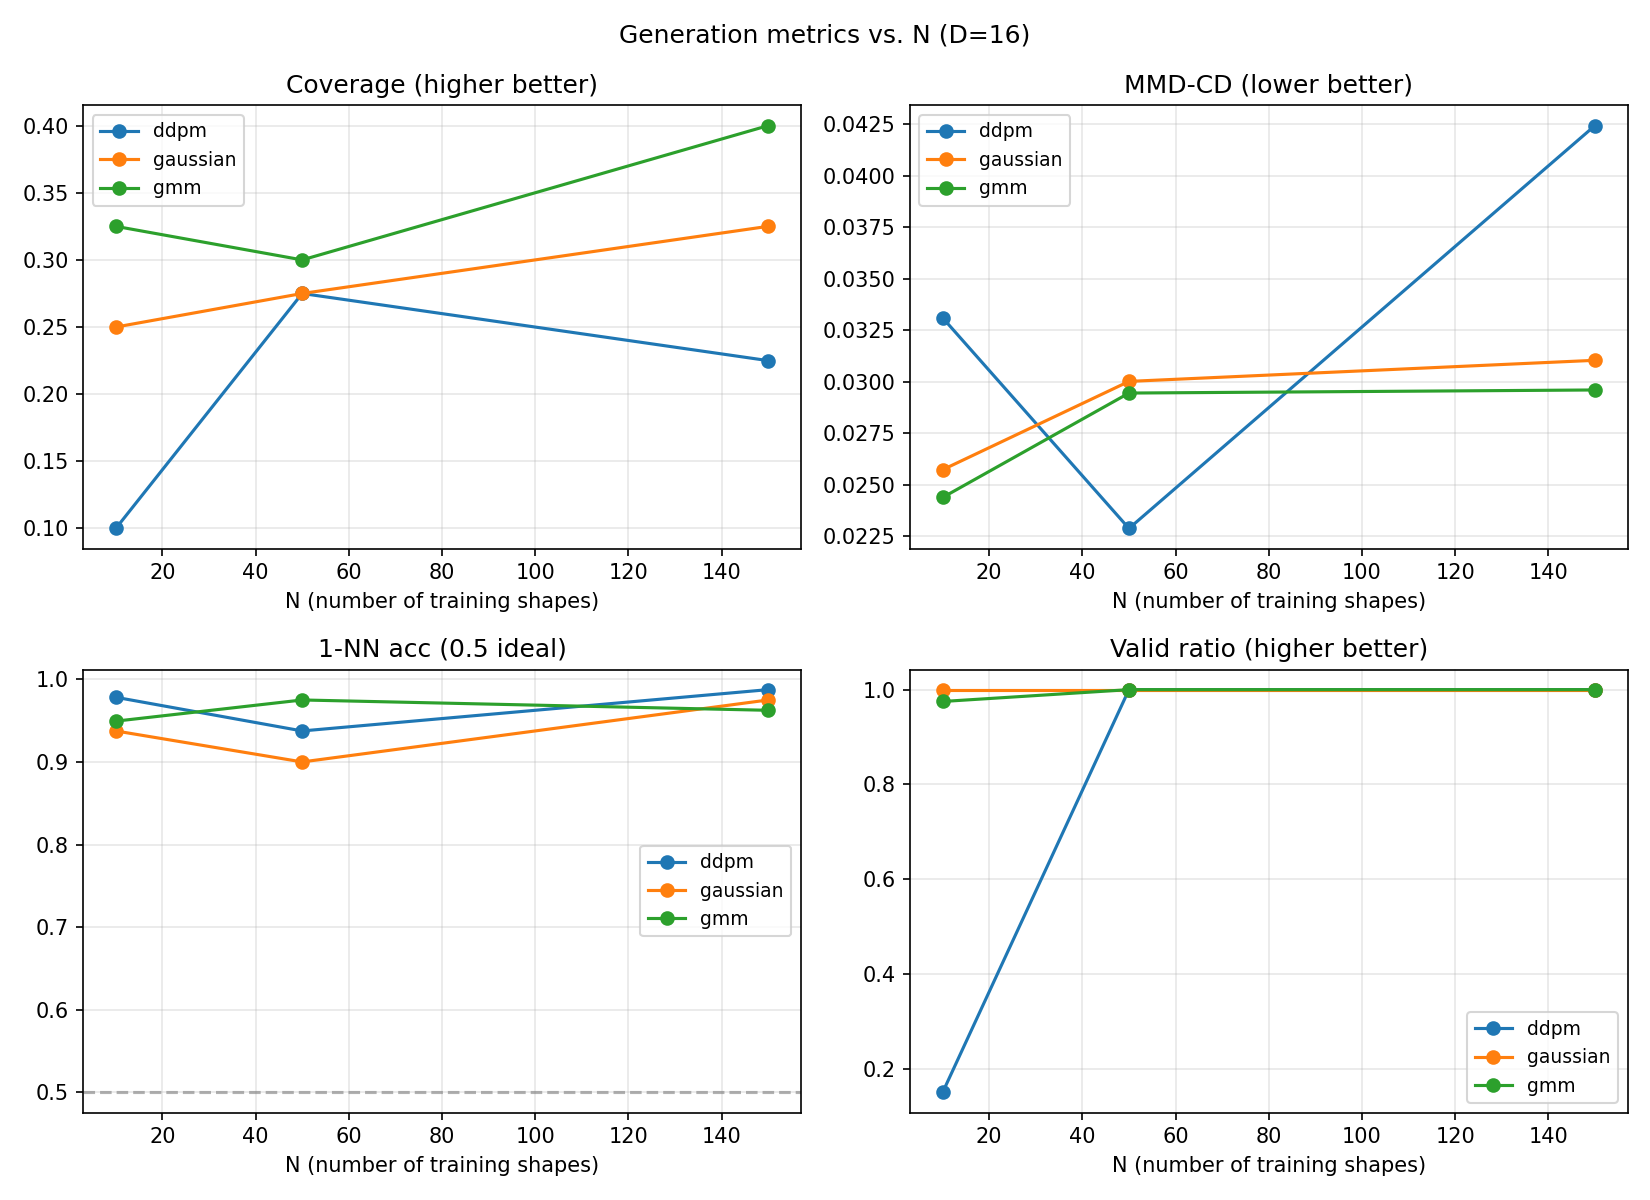
\includegraphics[width=\textwidth]{degradation_generation.png}
\caption{Generation metrics vs.\ number of training shapes $N$, per generator,
at the fixed latent dimension $D=16$. The dashed line marks the ideal 1-NN
accuracy of $0.5$.}
\label{fig:degradation}
\end{figure*}

\begin{figure*}[t]
\centering

\includegraphics[width=\textwidth]{degradation_reconstruction.png}
\caption{Reconstruction Chamfer distance and IoU vs.\ $N$ at $D=16$.}
\label{fig:recon}
\end{figure*}

\begin{figure*}[t]
\centering
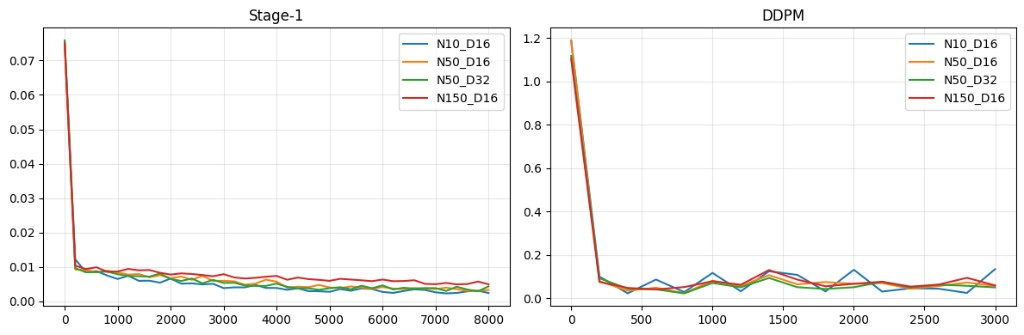
\includegraphics[width=\textwidth]{loss_curves.png}
\caption{Stage-1 clamped-$L_1$ reconstruction loss and Stage-2 DDPM
noise-prediction loss for each cell.}
\label{fig:loss}
\end{figure*}

\begin{figure*}[t]
\centering
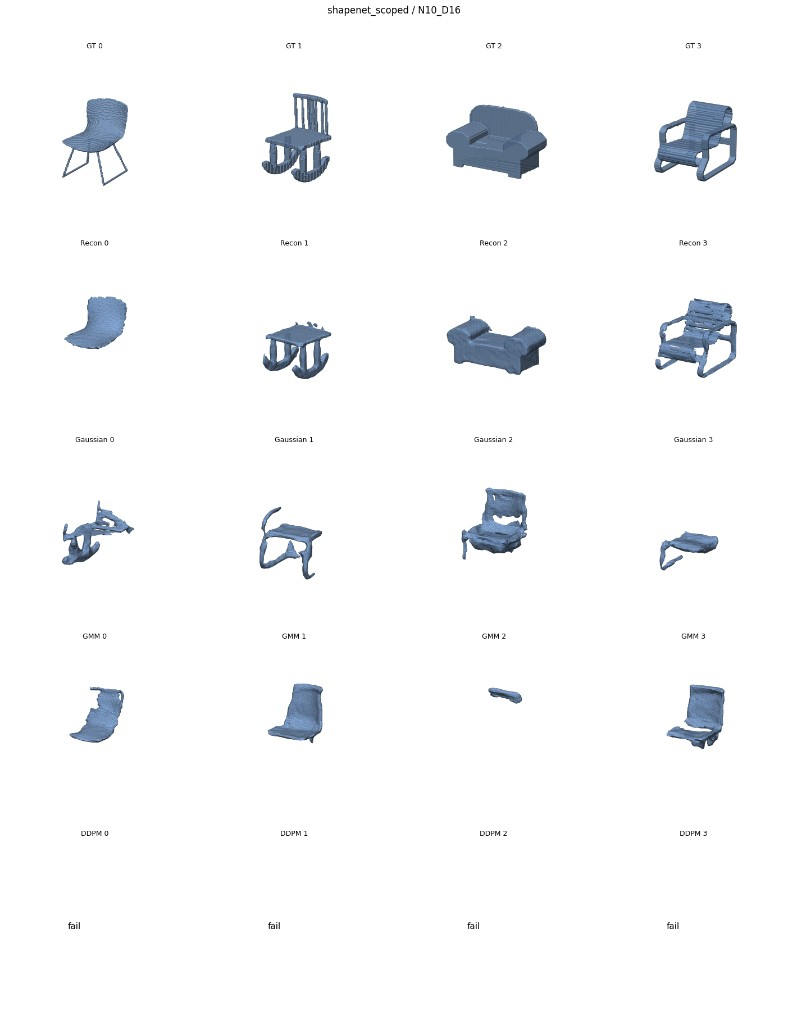
\includegraphics[width=\textwidth]{gallery.png}
\caption{Qualitative ShapeNet results at $N=10$, $D=16$, rendered as shaded
solids. Rows: ground-truth chair, reconstruction from its learned code, then
samples from the Gaussian, GMM, and DDPM priors. Reconstructions keep the coarse
silhouette but lose thin structure (the legs of column~1). Every DDPM sample
failed to produce a surface, which is the $0.15$ valid ratio of
\cref{tab:results} made visible; failed decodes are labelled rather than omitted.}
\label{fig:gallery}
\end{figure*}

\subsection{Ablation: latent dimension}
\label{sec:ablation}
The final block of \cref{tab:results} reports the $D=32$ cell at $N=50$, to be
compared against the $D=16$ cell at the same $N$. Doubling the latent dimension
doubles the per-shape capacity available to Stage~1 while leaving the decoder and
the training budget unchanged, so it is the cheapest available test of whether the
codes --- rather than the decoder --- were the bottleneck.

The two halves of the pipeline answer in opposite directions. Reconstruction
improves substantially: Chamfer falls from $0.0361$ to $0.0145$ and IoU rises from
$0.736$ to $0.814$, the best reconstruction of any cell in the study. Generation
does not follow. Coverage drops for every prior ($0.275 \to 0.225$ Gaussian,
$0.300 \to 0.225$ GMM, $0.275 \to 0.250$ DDPM), and the DDPM degrades sharply,
with MMD more than doubling ($0.0229 \to 0.0506$) and its valid ratio falling from
$1.00$ to $0.85$. Only the GMM's MMD improves ($0.0294 \to 0.0279$), by a margin
smaller than the spread across $N$.

This is the trade-off one expects once Stage~1 is healthy. Wider codes give
Stage~1 more room per shape, but Stage~2 then has to do density estimation in
$\mathbb{R}^{32}$ from the same $50$ points, and the diffusion model --- the most
parameter-hungry of the three and the one with the least inductive bias --- pays
the largest price for it.

\subsection{Discussion}

\paragraph{How much of the budget reaches the surface.} Two quantities have to be
read together in \cref{tab:results}. Reconstruction Chamfer/IoU bound what
\emph{any} prior can achieve, because a sampled code is decoded by the same
network: if the training codes themselves do not decode cleanly, no prior over
those codes can. The valid ratio then says how often a sampled code produces an
extractable surface at all. A generator can look strong on Coverage and MMD while
quietly failing on a large fraction of its samples, since those metrics are
computed only over samples that yielded a mesh. We therefore treat valid ratio as
a first-class result rather than a diagnostic.

Reconstruction is adequate across the sweep --- Chamfer $0.0122$--$0.0361$ and IoU
$0.683$--$0.784$ at $D=16$ --- so Stage~1 is not the binding constraint on the
comparison. The valid ratio is where the priors separate. It is $1.00$ in nine of
the twelve generator/cell combinations, and every exception belongs to a
non-Gaussian prior: the GMM once, mildly ($0.975$ at $N=10$), and the DDPM twice,
severely ($0.85$ at $D=32$, and $0.15$ at $N=10$). That last number is the one the
argument above was written for. The DDPM's Coverage and MMD at $N=10$ are computed
over the six samples that produced a surface out of forty, so they are not
comparable to the other rows; reported alone they would understate the failure by
roughly an order of magnitude.

\paragraph{Do the priors differ at all?} This is the paper's question, and the
informative outcome may well be a negative one. At small $N$ the empirical code
distribution is a handful of points in $\mathbb{R}^{16}$; a full-covariance
Gaussian already has $D + D(D{+}1)/2 = 152$ parameters to fit
$N$ vectors, so the mixture and the diffusion model are being asked to find
structure in a sample that may not support it. If the three priors are within
noise of each other, the practical conclusion is that diffusion's extra machinery
buys nothing in this regime --- which is precisely the claim the proposal set out
to test, and it inverts the usual reading of 3D-LDM's result by showing where its
advantage comes from (scale) rather than disputing it.

The outcome is negative for diffusion, but not in the way anticipated: the priors
do differ, and the ordering is consistent and against the DDPM. On Coverage the
GMM leads at every $N$ and the ranking GMM $\ge$ Gaussian $>$ DDPM holds in two of
three cells (the three tie within $0.025$ at $N=50$). On MMD the Gaussian and GMM
sit in a narrow band, $0.0244$--$0.0310$, that is comparable to the change induced
by varying $N$; the DDPM produces both the best value in the study ($0.0229$ at
$N=50$) and by some margin the worst ($0.0424$ at $N=150$, $0.0506$ at $D=32$),
which is the signature of a high-variance estimator rather than a better one. The
Gaussian--GMM gap is real but modest: the GMM's Coverage advantage over the
Gaussian is $0.075$, $0.025$, and $0.075$, always in the same direction but of the
same order as the spread across $N$. So the honest reading is that a mixture is
worth its two extra lines over a single Gaussian, and that the diffusion model,
which costs an entire second training loop, is not merely unhelpful here but
actively harmful at the extremes of the sweep.

\paragraph{The 1-NN sanity check.} 1-NN accuracy is the strictest of the three
generation metrics: $0.5$ means a classifier cannot tell generated shapes from
real ones, and values near $1.0$ mean it always can. Under a budget of $40$
samples against $40$ references, and with reconstructions that are themselves
imperfect, we expect values far above $0.5$ --- a reminder that Coverage and MMD
alone can flatter a generator whose samples are individually implausible.

Observed 1-NN accuracy spans $0.900$--$0.988$ and no generator comes close to
$0.5$: the best value in the study is the Gaussian at $N=50$ ($0.900$), and eight
of the twelve rows exceed $0.93$. Generated and real chairs therefore remain
trivially separable in every configuration we ran, which bounds how much weight
the Coverage and MMD comparisons can carry. The ranking above describes degrees of
failure, not a contest between models that work. This is the metric most
responsive to reconstruction quality rather than to the prior, and it is
consistent with a gallery in which samples are chair-\emph{like} without being
chairs.

\paragraph{Trend with $N$.} More shapes cut two ways here. The prior sees a larger
sample, which should help it, but Stage~1 must fit more geometry with a fixed
decoder and a fixed iteration budget, which should hurt reconstruction --- and
reconstruction quality caps everything downstream. \Cref{fig:degradation} and
\cref{fig:recon} separate these effects.

Both effects appear, and for the two classical priors the prior-side gain wins.
Reconstruction IoU falls monotonically as $N$ grows, $0.784 \to 0.736 \to 0.683$,
exactly the fixed-capacity story. Yet Coverage rises over the same range for the
Gaussian ($0.250 \to 0.325$) and the GMM ($0.325 \to 0.400$): a better-estimated
prior more than compensates for a slightly worse decoder. The DDPM does not share
this, improving sharply from $N=10$ to $N=50$ ($0.100 \to 0.275$, and $0.15 \to
1.00$ valid) and then degrading at $N=150$ ($0.225$) --- its problem is not sample
size alone.

Reconstruction Chamfer is not monotone ($0.0151$, $0.0361$, $0.0122$), and we read
the IoU trend as the reliable one. Chamfer here is an unbounded average over only
ten shapes, so a single poor decode can dominate it, whereas IoU is bounded in
$[0,1]$ and cannot be moved as far by one outlier. Reporting both is what makes
the discrepancy visible; either metric alone would have told a tidier story than
the data supports.

\paragraph{Latent dimension.} \Cref{sec:ablation} compares $D=32$ against $D=16$
at $N=50$ under the repaired pipeline: it helps Stage~1 (IoU $0.736 \to 0.814$)
and hurts Stage~2 (Coverage down for all three priors). The comparison worth
drawing out is with the pre-repair measurement that motivated fixing $D=16$ in the
first place, where the same change moved Chamfer from $0.129$ to $0.540$. That
result does not reproduce. Under corrected labels the sign flips and $D=32$ gives
the best reconstruction in the study.

We take this as further evidence for the diagnosis of \cref{sec:watertight} rather
than as noise. The pre-repair pipeline rewarded capacity for fitting a sign field
that was largely arbitrary near the surface, so more capacity meant a better fit to
worse labels --- the same inversion as the decoder-width result in
\cref{sec:failure-modes}. Once the labels describe a closed solid, capacity behaves
as one would expect on the axis it should help. The honest caveat is that this
also weakens the original justification for the scoped design, and that we
re-tested only the latent dimension: the width-$512$ decoder was never re-run
post-repair, so we cannot claim the width result inverts too, only that we no
longer have reason to believe it as stated.

\paragraph{Qualitative gallery.} \Cref{fig:gallery} is the check that the metrics
cannot provide. Chamfer distance between surface point clouds is fairly forgiving
of a shape that has roughly the right mass in roughly the right places, so a
recognizable chair and a plausible-but-wrong blob can score similarly. Reading the
gallery alongside the table is what caught the label bug of
\cref{sec:watertight} in the first place: the numbers were unremarkable while the
meshes were fragments. Failed decodes are drawn as an explicit \emph{fail} marker
rather than silently omitted, so the figure and the valid ratio agree.

What \cref{fig:gallery} shows is a pipeline that has crossed from incoherent to
coarse. Ground-truth chairs are cleanly repaired solids, and reconstructions
recover the seat-and-back massing while losing thin structure: the sled legs of
the first column disappear, and the slatted back of the second becomes a plate.
That is the visual counterpart of a $D=16$ code and a $48^3$ extraction grid, and
it is what caps 1-NN accuracy well above $0.5$. Samples from the Gaussian and GMM
priors are chair-like in silhouette and clearly varied --- seats, backs, and
armrest-like masses in plausible relative positions --- but they are not chairs;
several have holes or detached fragments, which is why they can score reasonable
Coverage while remaining trivially separable from real shapes. There is no visible
mode collapse: distinct samples remain distinct, consistent with Coverage that
rises rather than saturates. The DDPM row contains no geometry at all, every one
of its four samples having failed to cross zero. That is the clearest statement of
the paper's result: at $N=10$, the two priors that assume a shape for the code
distribution still produce chairs, and the one that tries to learn the shape from
ten examples produces nothing.

\section{Conclusion}
We compared Gaussian, GMM, and DDPM priors over frozen DeepSDF codes on a
ShapeNet chair subset as the dataset shrank, $N \in \{10,50,150\}$ at $D=16$,
with $D=32$ ablated separately. The goal was not state of the art but a
controlled answer to when diffusion is worth its complexity on real meshes under
a modest compute budget.

It is not worth it at this scale. The GMM gave the best Coverage at every $N$
($0.325$, $0.300$, $0.400$) with the Gaussian just behind, while the DDPM won no
cell, was worst on every generation metric at $N=150$, and at $N=10$ decoded to a
surface only $15\%$ of the time against $100\%$ for the Gaussian. Its one strength,
the best MMD in the study at $N=50$ ($0.0229$), sits alongside the two worst
($0.0424$ and $0.0506$), which reads as variance rather than capability. The
ranking is also not close to a contest between working models: 1-NN accuracy never
fell below $0.900$ against an ideal of $0.5$, so what we are ranking is degrees of
failure. Read against 3D-LDM, this locates the benefit of latent diffusion in the
data scale it was demonstrated at rather than in the mechanism itself.

The most transferable lesson is not about the priors at all. The failure that
dominated our results presented as an \emph{optimization} problem while actually
being a data problem: non-watertight input meshes corrupting the SDF sign that
DeepSDF trains on (\cref{sec:watertight}). Its most confusing symptom was that
added capacity simultaneously lowered training loss and worsened extracted geometry
(\cref{sec:failure-modes}) --- an inversion that vanished once the labels were
repaired, as the latent-dimension ablation confirms. The training loss, the
quantity one naturally monitors, moved in the reassuring direction throughout. On a
pipeline that ends in Marching Cubes, point-wise loss is a weak proxy for the
surface, and geometry has to be inspected directly.

Limitations include the cost of mesh repair, the sensitivity of Marching Cubes to
under-trained fields, the single synset, and the modest sample counts behind the
generation metrics ($40$ samples against $40$ references), which limits how
finely Coverage and 1-NN accuracy can be resolved. Future work could scale $N$
within the chairs category, retune the optimizer for wider decoders instead of
fixing width, and add flow-based priors as a fourth point on the
minimal-to-expressive spectrum.

\small
\setlength{\bibsep}{1pt}
\bibliography{references}
\bibliographystyle{acl_natbib}
\normalsize

\appendix
\onecolumn
\section{Original Proposal}
The approved project proposal is reproduced below.
% Approved proposal, reproduced verbatim (see Final_Project/proposal.md).
\paragraph{Title.} Generative Latent Models for DeepSDF: Gaussian vs Diffusion
in the Small-Data Regime. \emph{Author:} Amit Benbenishti.

\paragraph{Problem definition.} DeepSDF learns one latent code per shape, but
does not learn a distribution over codes---random codes decode to invalid
shapes. I train a generative model over the latent space (not over shapes
directly) and study which simple prior works when data and capacity are limited.

\paragraph{Approach.} \emph{Stage 1:} train a DeepSDF auto-decoder on a shape
collection; collect latent codes $\{z_i\}$. \emph{Stage 2 (frozen decoder):} fit
two generators on $\{z_i\}$---(1) Gaussian (mean + covariance), (2) DDPM
diffusion over $z$ (same noise-prediction setup as HW3, applied to vectors).
\emph{Inference:} sample $z$ from a generator $\rightarrow$ decode with
$f(z, x) \rightarrow$ SDF $\rightarrow$ mesh. Sweep $N \in \{10, 50, 150\} \times
D \in \{16, 32\}$ and compare generators. Goal is not SOTA---it is to identify
when diffusion is worth the extra complexity over a Gaussian. All training code
is my own.

\paragraph{Motivation.} 3D-LDM uses latent diffusion over DeepSDF codes at full
ShapeNet scale; naive Gaussian sampling from the same latent space often fails.
I study the minimal-resource regime (small $N$, small $D$, Colab) where that
tradeoff is unknown.

\paragraph{Validation.} \emph{Data:} ShapeNet subset ($\sim$50--200 meshes) or
synthetic shapes + \texttt{stanford\_bunny.obj}. \emph{Metrics:} Chamfer + IoU
(reconstruction); Coverage, MMD, 1-NN accuracy (generation); qualitative samples
and interpolations. \emph{Mid-point checks:} (1) overfit one shape, (2) train
DeepSDF on $\sim$10 shapes and extract codes, (3) sample one mesh from Gaussian
and one from diffusion. \emph{Final:} full $N\times D$ grid + generator
comparison + degradation curves, including negative results (e.g., Gaussian
matches diffusion at small $N$).

\paragraph{Related work.} DeepSDF~\citep{park2019deepsdf}---auto-decoder and
latent codes (Stage 1). 3D-LDM~\citep{nam2022lion3dldm}---latent diffusion over
DeepSDF codes at scale; does not study small $N/D$ or Gaussian vs diffusion
explicitly. DreamFusion / DDPM~\citep{poole2022dreamfusion, ho2020ddpm}---
diffusion training (HW3 connection).


\end{document}
